\documentclass[tikz,border=10pt]{standalone}
\begin{document}
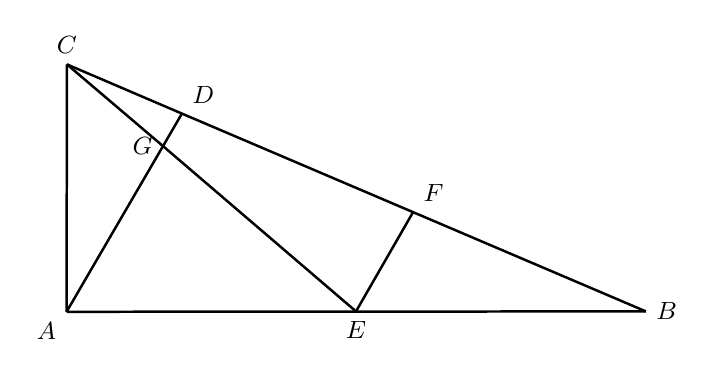
\begin{tikzpicture}[line width=0.9pt, line join=round,
  every node/.style={font=\fontsize{9}{10.8}\selectfont}]
\coordinate (A) at (-3.686,-1.570);
\coordinate (B) at (3.671,-1.565);
\coordinate (C) at (-3.681,1.572);
\coordinate (D) at (-2.221,0.947);
\coordinate (F) at (0.715,-0.304);
\coordinate (G) at (-2.461,0.534);




\coordinate (E) at (-0.010,-1.565);


\draw (A) -- (B);
\draw (C) -- (A);


\draw (C) -- (D) -- (B);


\draw (A) -- (G) -- (D);
\draw (C) -- (G) -- (E);


\draw (E) -- (F);


\node[below left] at (A) {$A$};
\node[right] at (B) {$B$};
\node[above] at (C) {$C$};
\node[above right] at (D) {$D$};
\node[below] at (E) {$E$};
\node[above right] at (F) {$F$};
\node[left] at (G) {$G$};
\end{tikzpicture}
\end{document}